\chapter{Scaling Your Practice with Automation}

%! suppress = LineBreak
\begin{warningblock}
    This is an Early Release. You're getting the raw and unedited content as I write. I'm doing this, so you can take advantage of the content
    before the official release, AND you can share critical feedback (plus, I include you in the credits of the official release)
    To get notified when I add new section(s), \href{https://discord.gg/X2USgYTB}{join the Business Automators discord community}
\end{warningblock}
\begin{importantblock}
    If you found a problem, \href{https://discord.gg/X2USgYTB}{drop a comment in the discord community} or  \href{mailto:dele@protomated.com}{email dele@protomated.com}.
\end{importantblock}


%
%

As an IT consultant, you've mastered the art of solving complex technical problems for your clients. But how do you take your practice to the next level? The answer lies in strategic automation. In this chapter, we'll explore how to create an automation roadmap, price your automated services effectively, and learn from a real-world case study of explosive growth through automation.

\section{Creating Your Automation Roadmap}

An automation roadmap is your strategic plan for implementing automation across your practice. Let's break down the process into manageable steps:

\subsection{Step 1: Identify Automation Candidates}

Begin by listing all the processes in your practice.\ Consider:
\begin{itemize}
    \item Client onboarding
    \item Project management
    \item Reporting and analytics
    \item Billing and invoicing
    \item Customer support
    \item Marketing and lead generation
\end{itemize}

% TODO @illustrate: Illustration of a mind map showing different areas of a consulting practice

\subsection{Step 2: Prioritize Processes}

Not all processes are created equal. Prioritize based on:
\begin{itemize}
    \item Potential time savings
    \item Impact on client satisfaction
    \item Complexity of automation
    \item Frequency of the process
\end{itemize}

Create a matrix to visualize priority:

% TODO @illustrate: 2x2 matrix with "Impact" on one axis and "Effort" on the other

\subsection{Step 3: Stakeholder Alignment}

Identify key stakeholders in your practice and get their buy-in. This might include:
\begin{itemize}
    \item Team members who will use the automated systems
    \item Clients who will be affected by the changes
    \item Partners or vendors involved in your processes
\end{itemize}

\subsection{Step 4: Process Deep Dive}

For each prioritized process, conduct a thorough analysis:

1. \textbf{Document the current workflow}:
   \begin{itemize}
     \item Interview team members involved in the process
     \item Create a step-by-step breakdown of the current workflow
     \item Identify inputs, outputs, and decision points
   \end{itemize}

2. \textbf{Identify pain points and inefficiencies}:
   \begin{itemize}
     \item Look for bottlenecks and delays
     \item Identify manual, repetitive tasks
     \item Note areas prone to errors or inconsistencies
   \end{itemize}

3. \textbf{Envision the ideal automated workflow}:
   \begin{itemize}
     \item Brainstorm how automation could address each pain point
     \item Consider how to streamline decision points
     \item Think about potential integrations with existing systems
   \end{itemize}

4. \textbf{Map the process visually}:
   We recommend using Excalidraw (https://excalidraw.com/) for this step. Excalidraw is a free, open-source tool that allows for easy creation and sharing of diagrams. Its simple interface is perfect for quickly mapping out processes and collaborating with your team.

Here's an example of what that might look like:

\begin{figure}[H]
    \centering
    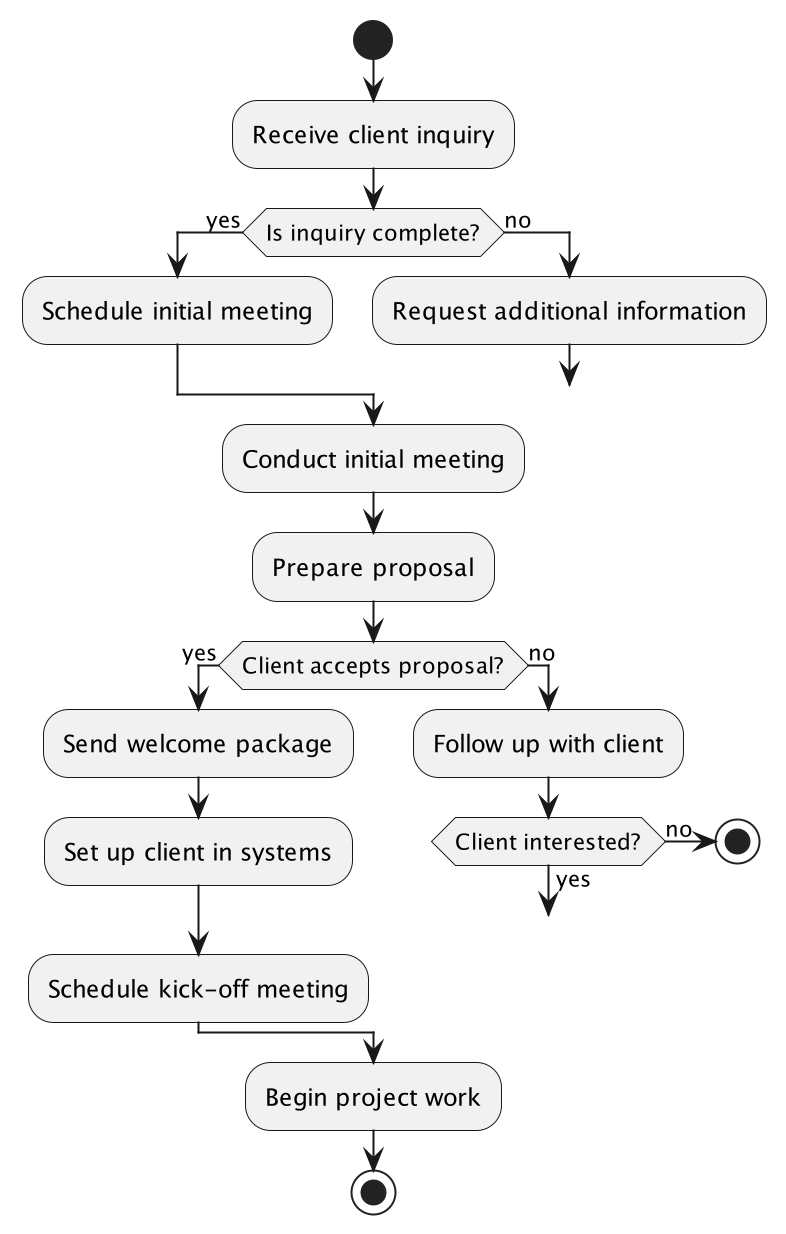
\includegraphics[width=0.5\textwidth]{figures/04-automation-roadmap-process}
    \caption{An example mapping a client onboarding process}
    \label{fig:client-automation-mapping-example}
\end{figure}

\subsection{Step 5: Select Technology Partners}

Based on your needs, choose the right tools. Consider:

1. \textbf{n8n for workflow automation}:
   \begin{itemize}
     \item Open-source and self-hostable, providing full control over your data
     \item Highly flexible, allowing for complex workflow creation
     \item Cost-effective, with a free self-hosted option and reasonable cloud pricing
     \item Enables integration with a wide range of services and APIs
   \end{itemize}

2. \textbf{NoCoDB for database management}:
   \begin{itemize}
     \item Open-source alternative to Airtable, offering data sovereignty
     \item Provides a user-friendly interface for managing complex data
     \item Can be self-hosted, ensuring data privacy and reducing costs
     \item Allows for easy creation of views and forms for data entry
   \end{itemize}

3. \textbf{BudiBase for creating custom applications}:
   \begin{itemize}
     \item Open-source low-code platform, allowing for rapid application development
     \item Can be self-hosted, ensuring control over your applications and data
     \item Offers a range of pre-built components to speed up development
     \item Integrates well with various data sources, including NoCoDB
   \end{itemize}

4. \textbf{Integration capabilities with your existing tools}:
   \begin{itemize}
     \item Ensure chosen tools can integrate with your current tech stack
     \item Look for native integrations or API accessibility
     \item Consider using n8n as a central hub for connecting various tools
   \end{itemize}

These tools offer significant value in terms of cost and data privacy:
\begin{itemize}
  \item \textbf{Cost}: All are open-source with self-hosting options, reducing licensing costs
  \item \textbf{Data Privacy}: Self-hosting ensures your client data never leaves your control
  \item \textbf{Customization}: Open-source nature allows for tailoring to your specific needs
  \item \textbf{Scalability}: These tools can grow with your practice without prohibitive costs
\end{itemize}

\subsection{Step 6: Develop Your Solution}

When developing your automated solution:

1. \textbf{Start with a Minimum Viable Automation (MVA)}:
   \begin{itemize}
     \item Focus on automating the core functionality first
     \item Aim for a working solution that can be tested and improved upon
     \item Get early feedback to guide further development
   \end{itemize}

2. \textbf{Use modular design for scalability}:
   \begin{itemize}
     \item Break down complex workflows into smaller, reusable components
     \item Design with future expansion in mind
     \item Use version control (e.g., Git) to manage your automation code
   \end{itemize}

3. \textbf{Document your automation thoroughly}:
   \begin{itemize}
     \item Create clear, step-by-step documentation for each automated process
     \item Include setup instructions, dependencies, and troubleshooting guides
     \item Use tools like Outline (recommended below) to organize documentation
   \end{itemize}

\subsection{Step 7: Rigorous Testing}

Implement a comprehensive testing strategy:

1. \textbf{Unit testing for individual components}:
   \begin{itemize}
     \item Test each node or step in your n8n workflows independently
     \item Verify that individual functions in BudiBase apps work as expected
     \item Ensure data validation in NoCoDB is functioning correctly
   \end{itemize}

2. \textbf{Integration testing for connected systems}:
   \begin{itemize}
     \item Test entire workflows end-to-end
     \item Verify data flows correctly between different tools (e.g., n8n to NoCoDB to BudiBase)
     \item Simulate various scenarios, including error conditions
   \end{itemize}

3. \textbf{User acceptance testing with your team}:
   \begin{itemize}
     \item Have team members who will use the system test it in real-world scenarios
     \item Gather feedback on usability and functionality
     \item Identify any training needs for effective use of the new systems
   \end{itemize}

4. \textbf{Performance and security testing}:
   \begin{itemize}
     \item Test system performance under expected load
     \item Conduct security audits, especially for self-hosted solutions
     \item Verify data encryption and access controls are working as intended
   \end{itemize}

\subsection{Step 8: Pilot Program}

Run a pilot with a subset of your clients or projects:

1. \textbf{Select diverse pilot participants}:
   \begin{itemize}
     \item Choose clients of varying sizes and industries
     \item Include both tech-savvy and less technical clients
     \item Aim for a mix of new and long-standing client relationships
   \end{itemize}

2. \textbf{Set clear success metrics}:
   \begin{itemize}
     \item Define quantitative metrics (e.g., time saved, error reduction)
     \item Include qualitative measures (e.g., client satisfaction, ease of use)
     \item Establish baseline measurements for comparison
   \end{itemize}

3. \textbf{Gather detailed feedback}:
   \begin{itemize}
     \item Conduct regular check-ins with pilot participants
     \item Use surveys and interviews to collect comprehensive feedback
     \item Encourage reporting of any issues or suggestions for improvement
   \end{itemize}

4. \textbf{Iterate based on pilot results}:
   \begin{itemize}
     \item Analyze feedback and performance data
     \item Make necessary adjustments to your automated solutions
     \item Consider running multiple pilot iterations for critical systems
   \end{itemize}

% TODO @template: Downloadable template for creating an automation roadmap

\section{Pricing and Packaging Automated Services}\label{sec:pricing-and-packaging-automated-services}

Effectively monetizing your automated services is crucial for scaling your practice. Let's explore the best pricing strategies for small IT consulting firms.

\subsection{Top 3 Pricing Models for Automated Services}

1. \textbf{Tiered Subscription Model}
   \begin{itemize}
     \item \textbf{Description}: Offer different levels of service (e.g., Basic, Pro, Enterprise)
     \item \textbf{Pros}:
       \begin{itemize}
         \item Provides predictable recurring revenue
         \item Allows clients to choose a level that fits their needs and budget
         \item Easier to upsell clients to higher tiers over time
       \end{itemize}
     \item \textbf{Cons}:
       \begin{itemize}
         \item May leave money on the table with high-value clients
         \item Can be complex to determine what features go in each tier
       \end{itemize}
     \item \textbf{Implementation Strategy}:
       \begin{itemize}
         \item Start with 3 tiers: Basic, Pro, and Enterprise
         \item Clearly define what automations and services are included in each tier
         \item Consider offering a discount for annual subscriptions
       \end{itemize}
   \end{itemize}

2. \textbf{Value-Based Pricing}
   \begin{itemize}
     \item \textbf{Description}: Price based on the value delivered to the client
     \item \textbf{Pros}:
       \begin{itemize}
         \item Can lead to higher prices for high-impact automations
         \item Aligns your incentives with client outcomes
         \item Differentiates you from competitors who use cost-plus pricing
       \end{itemize}
     \item \textbf{Cons}:
       \begin{itemize}
         \item Requires clear demonstration of ROI
         \item Can be challenging to quantify value for some services
         \item May require more negotiation with clients
       \end{itemize}
     \item \textbf{Implementation Strategy}:
       \begin{itemize}
         \item Develop case studies showing the impact of your automations
         \item Create an ROI calculator for potential clients
         \item Consider performance-based pricing elements (e.g., bonuses for exceeding targets)
       \end{itemize}
   \end{itemize}

3. \textbf{Hybrid Model: Base + Usage}
   \begin{itemize}
     \item \textbf{Description}: Charge a base fee for setup and maintenance, plus usage-based fees
     \item \textbf{Pros}:
       \begin{itemize}
         \item Balances predictable income with scalability
         \item Allows for lower entry point while capturing upside
         \item Can be attractive to clients unsure of their usage needs
       \end{itemize}
     \item \textbf{Cons}:
       \begin{itemize}
         \item More complex to explain and implement
         \item May require sophisticated usage tracking
         \item Could lead to unpredictable revenue if usage varies greatly
       \end{itemize}
     \item \textbf{Implementation Strategy}:
       \begin{itemize}
         \item Set a competitive base fee that covers your core costs
         \item Define clear usage metrics (e.g., number of automated processes, data volume)
         \item Offer volume discounts to encourage higher usage
       \end{itemize}
   \end{itemize}

\subsection{Factoring in Setup and Maintenance Costs}

To make your services attractive while ensuring profitability:

1. Charge a lower upfront fee to reduce barriers to entry
2. Include ongoing maintenance costs in a monthly or annual subscription
3. Structure pricing to recover setup costs over the first 6-12 months of the engagement

\subsection{Effective Packaging Strategies}

Bundle automated services with traditional consulting to create compelling offers:

1. \textbf{The "Digital Transformation" Package}
\begin{itemize}
    \item Combine strategy consulting with implementation of key automations
    \item Offer ongoing support and optimization
\end{itemize}

2. \textbf{The "Efficiency Boost" Bundle}
\begin{itemize}
    \item Audit current processes and implement targeted automations
    \item Include training and change management support
\end{itemize}

3. \textbf{The "Scalability Suite"}
\begin{itemize}
    \item Focus on automations that enable client growth
    \item Tie pricing to client's growth metrics for alignment
\end{itemize}

Remember, the key is tsubsection{Step 4o demonstrate how your automated services amplify the value of your traditional consulting offerings.

\section{Case Study: From 5 to 50 Clients with No Additional Hires}

Let's examine how one IT consulting practice leveraged automation to achieve 10x growth without expanding their team.

\subsection{The Challenge}

Our case study firm faced several challenges common to small IT consultancies:
\begin{itemize}
    \item Staying profitable while scaling
    \item Attracting new clients in a competitive market
    \item Pricing services competitively while maintaining margins
    \item Staying ahead of rapidly evolving tech trends
    \item Demonstrating clear ROI to clients
    \item Managing and sharing internal knowledge effectively
\end{itemize}

\subsection{The Automation Strategy}

The firm implemented a comprehensive automation strategy:

1. \textbf{Client Onboarding Automation}
\begin{itemize}
    \item Used n8n to create a seamless onboarding workflow
    \item Reduced onboarding time from 2 weeks to 2 days
\end{itemize}

2. \textbf{Automated Reporting and Analytics}
\begin{itemize}
    \item Developed custom dashboards using BudiBase
    \item Provided real-time insights to clients, improving satisfaction
\end{itemize}

3. \textbf{Knowledge Management System}
\begin{itemize}
    \item Created a centralized, searchable knowledge base using Outline (https://www.getoutline.com/)
    \item Outline is an open-source, self-hostable wiki that integrates well with other tools
    \item Enabled rapid problem-solving and reduced duplicate work
    \item Improved team collaboration and preserved institutional knowledge
\end{itemize}

4. \textbf{Predictive Maintenance Alerts}
\begin{itemize}
    \item Implemented IoT sensors and n8n workflows for client infrastructures
    \item Proactively addressed issues before they impacted clients
\end{itemize}

5. \textbf{Automated Lead Nurturing}
\begin{itemize}
    \item Developed an n8n workflow integrated with Twenty CRM (https://twenty.com/)
    \item Twenty is an open-source, self-hostable CRM system
    \item Implemented lead scoring and personalized follow-ups
    \item Increased conversion rates by 150%
\end{itemize}

\subsection{Measurable Outcomes}

The impact of these automations was significant:

1. \textbf{Revenue Growth}: 500% increase over 18 months
2. \textbf{Cost Reduction}: Maintained the same headcount while 10x-ing client base
3. \textbf{Client Satisfaction}: NPS score improved from 45 to 82
4. \textbf{Efficiency}: Reduced average project delivery time by 40%

\subsection{Unexpected Benefits and Challenges}

\textbf{Benefits}:
\begin{itemize}
    \item Improved work-life balance for team members
    \item Attracted higher-quality clients due to advanced tech offerings
    \item Positioned the firm as a thought leader in automation
\end{itemize}

\textbf{Challenges}:
\begin{itemize}
    \item Initial resistance from some team members fearing job obsolescence
    \item Needed to upskill team in automation technologies
    \item Some clients required education on the benefeits of automation
\end{itemize}

\section{Conclusion}

Automation is not just a tool for efficiency; it's a catalyst for exponential growth in your IT consulting practice. By creating a thoughtful automation roadmap, pricing your services strategically, and learning from successful case studies, you can transform your practice and achieve remarkable scaling without proportionally increasing your workload or team size.

\textbf{Action Items}:\newline

\begin{enumerate}
    \item  Begin drafting your automation roadmap using the template provided. Identify your top three processes to automate and outline the potential impact on your practice.
    \item Join the Business Automator Discord channel to continue the conversation and connect with others on their automation journey: https://discord.gg/P6txNctp
    \item Download our comprehensive Automation Planning Workbook to help guide your journey.
\end{enumerate}

% TODO @qr: QR code for joining the Discord channel

% TODO @template: QR code for downloading the Automation Planning Workbook

By taking these steps, you'll be well on your way to scaling your IT consulting practice through the power of automation. Remember, the journey of automation is ongoing - continually reassess, refine, and expand your automated processes to stay ahead in the ever-evolving world of IT consulting.

